\fancyhead[C]{\normalsize\textbf{$\qquad$ Teil II: Multiple-Choice}}
\section*{Aufgabe 2 (33 Punkte)}
\vspace{0.4cm}
\subsection*{\frage{1}{3}}
In welchem Punkt hat die Funktion
\begin{align*}
	f(x,y) = 5x
\end{align*}
unter der Nebenbedingung
\begin{align*}
	\varphi(x,y) = 2 y^2 - x - 1 = 0
\end{align*}
ein Minimum?
\renewcommand{\labelenumi}{(\alph{enumi})}
\begin{enumerate}
	\item $ P= (-2,\sqrt{0.5}) $.
	\item $ P= (0,\sqrt{0.5}) $.
	\item $ P= (7,2) $.
	\item $ P= (-1,0) $.
	\item Keiner der oben gegebenen Punkte ist ein Minimum der Funktion $ f $ unter der Nebenbedingung $ \varphi(x,y)= 0 $.
\end{enumerate}
\ \\
\textbf{Lösung:}
\begin{mdframed}
\underline{\textbf{Vorgehensweise:}}
\renewcommand{\labelenumi}{\theenumi.}
\begin{enumerate}
\item Überlege dir, welche Punkte die Nebenbedingung erfüllen.
\item Nutze die Funktion (Darstellung einer Ellipse).
\end{enumerate}
\end{mdframed}

\underline{1. Überlege dir, welche Punkte die Nebenbedingung erfüllen}\\


\newpage

\subsection*{\frage{2}{3}}
Sei $ f $ eine zweimal stetig partiell differenzierbare Funktion zweier Variablen. Für den stationären Punkt $ (x_0,y_0) $ gilt:
\begin{align*}
	f_{xx}(x_0,y_0) < f_{yy}(x_0,y_0) < f_{xy}(x_0,y_0) < 0.
\end{align*} 
Dann gilt:
\renewcommand{\labelenumi}{(\alph{enumi})}
\begin{enumerate}
	\item $ f $ hat in $ (x_0,y_0) $ ein lokales Minimum.
	\item $ f $ hat in $ (x_0,y_0) $ ein lokales Maximum.
	\item $ f $ hat in $ (x_0,y_0) $ einen Sattelpunkt.
	\item Die Information genügt nicht, um zu entscheiden, ob $ f $ in $ (x_0,y_0) $ einen Sattelpunkt oder ein lokales Extremum hat.
\end{enumerate}
\ \\
\textbf{Lösung:}
\begin{mdframed}
	\underline{\textbf{Vorgehensweise:}}
	\renewcommand{\labelenumi}{\theenumi.}
	\begin{enumerate}
		\item .
	\end{enumerate}
\end{mdframed}
\underline{1. }\\
\newpage
\subsection*{\frage{3}{4}}
Die Funktion $ f $ sei gegeben durch
\begin{align*}
	f(x) = \int_2^{x^2} e^{\sin(t)} \ dt.
\end{align*}
Welcher der folgenden Ausdrücke gibt die Ableitung $ f^\prime(x) $ wieder?
\renewcommand{\labelenumi}{(\alph{enumi})}
\begin{enumerate}
	\item 
	$ f^\prime(x) = e^{\sin(x^2)} \sin(x^2)$.
	\item 
	$ f^\prime(x) = 2 x e^{\sin(x^2)}$.
	\item 
	$ f^\prime(x) = e^{\sin(x^2)}$.
	\item
	$ f^\prime(x) = 2 x e^{\sin(x^2)} \sin(x^2)$.
	\item 
	$ f^\prime(x) = x^2 e^{\sin(x^2)}$ 
	\item 
	Keiner der obigen Ausdrücke ist korrekt.
\end{enumerate}
\ \\
\textbf{Lösung:}
\begin{mdframed}
\underline{\textbf{Vorgehensweise:}}
\renewcommand{\labelenumi}{\theenumi.}
\begin{enumerate}
\item Verwende den Fundamentalsatz und die Kettenregel.
\end{enumerate}
\end{mdframed}

\underline{1. Verwende den Fundamentalsatz und die Kettenregel}\\
Wir definieren 
\begin{align*}
	g(x) = 
	\int_0^x e^{\sin(t)} \td{t}.
\end{align*}
Dann gilt $ f(x)  = g(x^2)$ und der Fundamentalsatz der Infinitismalrechnung liefert $ g^\prime(x) = e^{\sin(x)} $.
Mit der Kettenregel erhalten wir dann
\begin{align*}
	f^\prime(x) = g^\prime(x^2) \cdot \left(\frac{\mathrm{d}}{\mathrm{dx}} x^2\right)
	=
	e^{\sin(x^2)} \cdot 2x.
\end{align*}
Damit ist die Antwort (b) korrekt.

\newpage

\subsection*{\frage{4}{3}}
Sei $ f $ eine \textit{ungerade} Funktion, welche die folgenden drei (Integral-) Gleichungen erfüllt:
\begin{align*}
	\int_{-1}^9 f(x) \ dx = 15, \
	\int_4^9 f(x) \ dx = 5 \ \textrm{und} \
	\int_1^6 f(x) \ dx = 7.
\end{align*}
Dann ist der Wert des bestimmten Integrals
\begin{align*}
	\int_4^6 f(x) \ dx
\end{align*}  
gleich
\renewcommand{\labelenumi}{(\alph{enumi})}
\begin{enumerate}
	\item 
	$ 0 $.
	\item
	$ 3 $.
	\item
	$ 2 $.
	\item
	$ -3 $.
	\item
	Die Information genügt nicht, um den Wert des Integrals zu bestimmen.
\end{enumerate}\ \\
\textbf{Lösung:}
\begin{mdframed}
\underline{\textbf{Vorgehensweise:}}
\renewcommand{\labelenumi}{\theenumi.}
\begin{enumerate}
\item .
\end{enumerate}
\end{mdframed}

\underline{1. }\\
 

\newpage
\subsection*{\frage{5}{4}}
Gegeben ist die Funktion
\begin{align*}
	f(x) =
	\begin{cases}
		2 x c e^{1 - x^2}, \ &x \geq c  \geq 0\\
		\qquad	\ 0 , \ &x < c
	\end{cases}.
\end{align*}
$ f $ ist eine Dichtefunktion für
\renewcommand{\labelenumi}{(\alph{enumi})}
\begin{enumerate}
	\item 
	$ c = 0 $.
	\item 
	$ c = \frac{1}{e} $.
	\item 
	$ c= 1 $.
	\item 
	$ c = 2e $.
	\item
	alle $ c \in \mathbb{R}_{++} $.
\end{enumerate}
\ \\
\textbf{Lösung:}
\begin{mdframed}
\underline{\textbf{Vorgehensweise:}}
\renewcommand{\labelenumi}{\theenumi.}
\begin{enumerate}
\item .
\end{enumerate}
\end{mdframed}

\underline{1. }\\
 

\newpage

\subsection*{\frage{6}{3}}
Die quadratischen Matrizen $ A_{n \times n} $ und $ B_{n \times n} $ seien regulär.
Der Ausdruck
\begin{align*}
	(A B)^T(B^{-1} A^{-1})^T B (AB)^{-1}
\end{align*}
ist gleich
\renewcommand{\labelenumi}{(\alph{enumi})}
\begin{enumerate}
	\item 
	$ A^{-1} B $.
	\item 
	$ I $, die $ (n \times n) $ Einheitsmatrix.
	\item
	$ AB^{-1} $.
	\item
	$ B $.
	\item 
	$ A^{-1} $
\end{enumerate}
\ \\
\textbf{Lösung:}
\begin{mdframed}
\underline{\textbf{Vorgehensweise:}}
\renewcommand{\labelenumi}{\theenumi.}
\begin{enumerate}
\item .
\end{enumerate}
\end{mdframed}

\underline{1. }\\


\newpage
\subsection*{\frage{7}{2}}
\begin{center}
	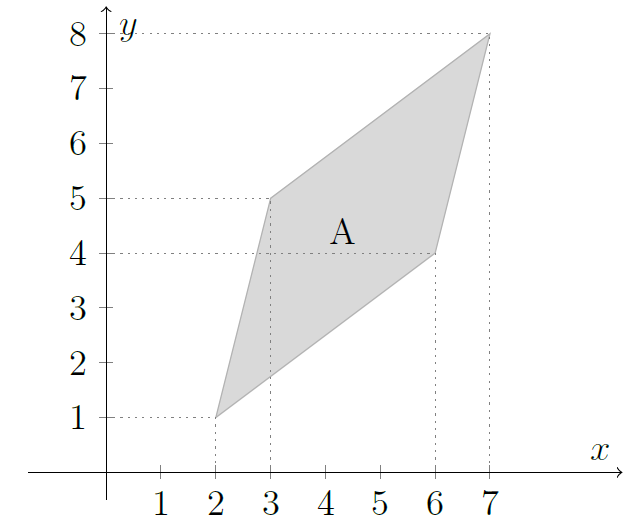
\includegraphics[width=0.7\textwidth]{pictures/aufgabe2_7}
\end{center}
Der Flächeninhalt $ A $ des Parallelogramms in der obigen Figur ist gleich
\renewcommand{\labelenumi}{(\alph{enumi})}
\begin{enumerate}
	\item 
	$ A = 10 $.
	\item
	$ A = 14 $.
	\item
	$ A = 5 \cdot  \sqrt{17} $.
	\item
	$ A = 16 $.
	\item
	$ A = 13 $.
\end{enumerate}
\ \\
\textbf{Lösung:}
\begin{mdframed}
\underline{\textbf{Vorgehensweise:}}
\renewcommand{\labelenumi}{\theenumi.}
\begin{enumerate}
\item .
\end{enumerate}
\end{mdframed}

\underline{1. }\\

\newpage

\subsection*{\frage{8}{3}}
$ A $ sei eine $ (5 \times 5) $-Matrix gegeben durch
\begin{align*}
	A
	=
	\left[
	\textbf{a}_1,
	\textbf{a}_2,
	\textbf{a}_3,
	\textbf{a}_4,
	\textbf{a}_5
	\right].
\end{align*}
Sei 
\begin{align*}
	B =
	\left[
	\textbf{a}_1 - 3 \textbf{a}_2,
	\textbf{a}_2,
	\textbf{a}_3 + \textbf{a}_2 - \textbf{a}_5,
	-2 \textbf{a}_4,
	\textbf{a}_5
	\right].
\end{align*}
Dann gilt
\renewcommand{\labelenumi}{(\alph{enumi})}
\begin{enumerate}
	\item 
	$ \det(B) = -2 \det(A) $.
	\item
	$ \det(B) = \det(A) $.
	\item
	$ \det(B) = 6 \det(A) $.
	\item
	$ \det(B) = -\det(A) $.
	\item
	Es gibt im Allgemeinen keine Relation zwischen $ \det(A) $ und $ \det(B) $.
\end{enumerate}
\ \\
\textbf{Lösung:}
\begin{mdframed}
\underline{\textbf{Vorgehensweise:}}
\renewcommand{\labelenumi}{\theenumi.}
\begin{enumerate}
\item .
\end{enumerate}
\end{mdframed}

\underline{1. }\\

\newpage
\subsection*{\frage{9}{2}}
Die Matrix $ A $ ist eine $ (7 \times 4) $-Matrix mit Rang $ 4 $.
Man bekommt die Matrix $ B $, indem man bei $ A $ die dritte Spalte streicht.\\
\\
Dann folgt:
\renewcommand{\labelenumi}{(\alph{enumi})}
\begin{enumerate}
	\item 
	$ \mathrm{rg}(B) = 4 $.
	\item
	$ \mathrm{rg}(B) = 3 $.
	
	\item
	$ \mathrm{rg}(B) < 3 $.
	
	\item
	Die Informationen reichen nicht aus, den Rang von $ B $ zu bestimmen.
\end{enumerate}
\ \\
\textbf{Lösung:}
\begin{mdframed}
	\underline{\textbf{Vorgehensweise:}}
	\renewcommand{\labelenumi}{\theenumi.}
	\begin{enumerate}
		\item Verwende die lineare Unabhängigkeit. 
	\end{enumerate}
\end{mdframed}

\underline{1. Verwende die lineare Unabhängigkeit}\\
Der Rang einer Matrix $ A $ ist wie folgt definert:
\begin{align*}
	\mathrm{rg}(A) &:= \textrm{Anzahl der linear unabhängigen Spalten}\\
	&:=\textrm{Anzahl der linear unabhängigen Zeilen}.
\end{align*}
Die Definition über die Zeilen ist in dieser Aufgabe nicht relevant. Diese soll die Gleichheit von Spalten/Zeilenrang verdeutlichen.\\
\\
Wir wissen, dass die $ (7 \times 4) $-Matrix $ A $ den Rang $ 4 $ besitzt. 
Damit sind die $ 4 $ Spalten der Matrix $ A $ linear unabhängig 
Durch das Streichen der dritten Spalte sind die $ 3 $ verbliebenen Spalten der $ (7 \times 3) $-Matrix $ B $ linear unabhängig.
Dies gilt, da jede Teilmenge einer linear unabhängigen Menge linear unabhängig ist. Nach der Definiton des Ranges gilt somit $ \mathrm{rg}(B) = 3 $.\\
\\
Damit ist die Anwort (b) korrekt.\\
\\
Alternativ gilt: Da $ B $ drei linear unabhängige Spalten besitzt, folgt $ \mathrm{rg}(B) \geq 3 $. Da $ B $ eine $ (7 \times 3) $-Matrix ist, gilt auch
\begin{align*}
	\mathrm{rg}(B) \leq \min(7,3) = 3
\end{align*}
und somit $ \mathrm{rg}(B) = 3 $.


\newpage
\subsection*{\frage{10}{3}}
Welche der folgenden Aussagen ist \textit{falsch}?
\renewcommand{\labelenumi}{(\alph{enumi})}
\begin{enumerate}
	\item 
	Die Summe von zwei regulären Matrizen ist regulär
	\item
	Das Produkt von zwei singulären Matrizen ist singulär.
	
	\item
	Der Rang einer Matrix ist gleich dem Rang der Transponierten.
	\item
	Der Rang einer $ (n \times m) $-Matrix ist kleiner gleich $ n $, unabhängig davon, was $ m \in \mathbb{N} $ ist.
	\item 
	Die Summe zweier singulärer Matrizen kann regulär sein.
\end{enumerate}
\ \\
\textbf{Lösung:}
\begin{mdframed}
	\underline{\textbf{Vorgehensweise:}}
	\renewcommand{\labelenumi}{\theenumi.}
	\begin{enumerate}
		\item Finde ein geeignetes Gegenbeispiel. 
	\end{enumerate}
\end{mdframed}

\underline{1. Finde ein geeignetes Gegenbeispiel}\\
Angenommen $ A $ sei regulär. Dann gilt 
\begin{align*}
	A + (-A) = 0,
\end{align*}
wobei mit $ 0 $ die Nullmatrix gemeint ist. Diese ist wegen $ \det(0) = 0 $ singulär. Mit der Einheitsmatrix sieht dieses Beispiel wie folgt aus:
\begin{align*}
	I + (-I)
	=
	\begin{pmatrix}
		1 & 0 \\
		0 & 1
	\end{pmatrix}
	+
	\begin{pmatrix}
	 -1 & 0 \\
	 0 & -1
	\end{pmatrix}
	=
	\begin{pmatrix}
		0 & 0 \\
		0 & 0
	\end{pmatrix}.
\end{align*} 
Wegen $ \det(I) = \det(-I) = 1 $ liegen hier zwei reguläre Matrizen vor, deren Summe singulär ist.\\
\\
Damit ist die Antwort (a) korrekt.\\
\\
Alternativ lässt sich die richtige Antwort auch durch Ausschließen der wahren Aussagen finden:
\begin{enumerate}
	\item[(b)]
	Seien $ A, B $ singuläre Matrizen. Dann ist das Produkt wegen 
	\begin{align*}
		\det(A \cdot B) = \det(A) \cdot \det(B) = 0 \cdot 0 = 0
	\end{align*}
	singulär.
	\item[(c)] Der Zeilenrang einer Matrix ist gleich dem Spaltenrang der Matrix.
	\item[(d)] 
	Sei $ A $ eine $ (n\times m) $-Matrix. Dann gilt
	\begin{align*}
		\mathrm{rg}(A) \leq \min(n,m) \leq n.
	\end{align*}
	\item[(e)]
	Die reguläre Einheitsmatrix lässt sich durch
	\begin{align*}
		\begin{pmatrix}
			1 & 0\\
			0 & 1
		\end{pmatrix}
		= 
		\begin{pmatrix}
			1 & 0 \\
			0 & 0
		\end{pmatrix}
		+
		\begin{pmatrix}
			0 & 0 \\
			0 & 1
		\end{pmatrix}
	\end{align*}
	zerlegen. Die zwei Summanden sind jeweils singulär.
\end{enumerate}
